%%%%%%%%%%%%%%%%%%%%%%%%%%%%%%%%%%%%%%%%%%%%%%%%%%%%%%%%%%%%%%%
%
% Welcome to Overleaf --- just edit your LaTeX on the left,
% and we'll compile it for you on the right. If you open the
% 'Share' menu, you can invite other users to edit at the same
% time. See www.overleaf.com/learn for more info. Enjoy!
%
%%%%%%%%%%%%%%%%%%%%%%%%%%%%%%%%%%%%%%%%%%%%%%%%%%%%%%%%%%%%%%%
\documentclass{beamer}
\usetheme{Warsaw}
\setbeamersize{text margin left=3mm,text margin right=3mm} 

%Information to be included in the title page:
\title{The Alignment Problem}
\subtitle{How Can Machines Learn Human Values?}
\author{Based on the book by Brian Christian}
%\institute{Overleaf}
\date{2021}

\begin{document}

\frame{\titlepage}


\begin{frame}
\frametitle{Outline}
\tableofcontents
\end{frame}

%%%%%%%%%%%%%%%%%%%%%%%%%%%%%%%%%%%%%%%%%%%%%%%%%%%%%%%%%%%%%%%
\section{Introduction}

\begin{frame}
\frametitle{Why is this important?}
\emph{"There is a growing sense that more and more of the world is being turned over, in one way, or another, to mathematical and computational models. It is as if we are consumed by the task of putting the world - figuratively and literally - on autopilot."} Brian Christian
\end{frame}

\begin{frame}
\frametitle{What could possibly go wrong?}
In your groups think about what could possibly go wrong with our headline rush into AI?
\end{frame}

%%%%%%%%%%%%%%%%%%%%%%%%%%%%% Representation %%%%%%%%%%%%%%%%%%%%%%%%%%%%%%%%%%

\section[Representation]{Representation - are our data sets fit for purpose?}

\begin{frame}
Representation - are our data sets fit for purpose?
\end{frame}

%%%% Gorillas 

\begin{frame}
\frametitle{Case study 1: What do you think caused this error?}
\begin{center}
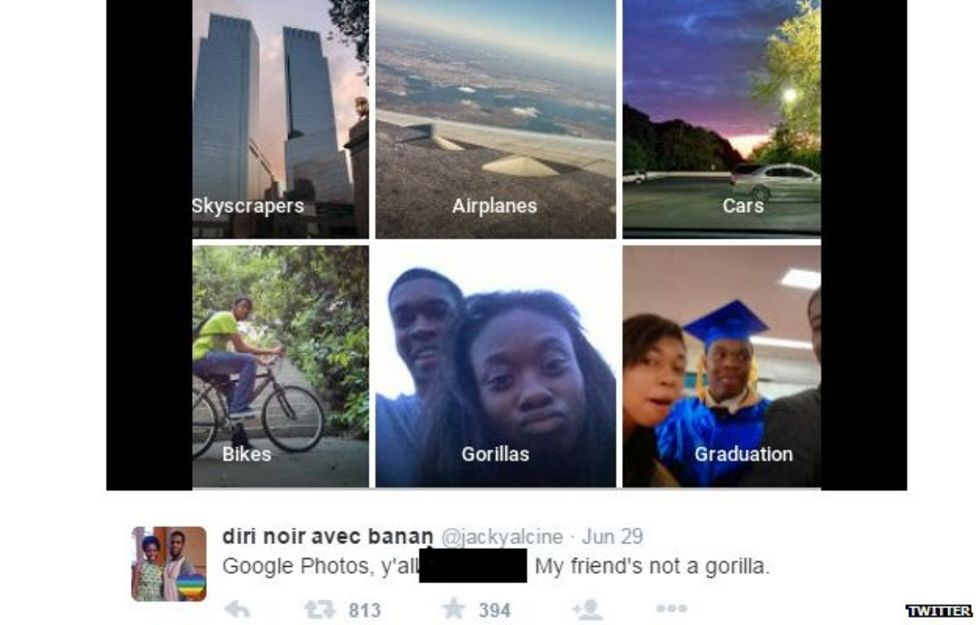
\includegraphics[width=0.65\textwidth]{./images/gorillas.jpg}
\end{center}
On Sunday evening of June 28, 2015, Jacky Alcine got a notification that a friend had uploaded a photo to Google Photos. It had created a new group for it and placed the photo in the new group. The group was titled 'Gorillas'.
\end{frame}

%%%% Face recognition


\begin{frame}
\frametitle{Face recognition and race 1}
\begin{columns}
    \begin{column}{0.3\textwidth}
        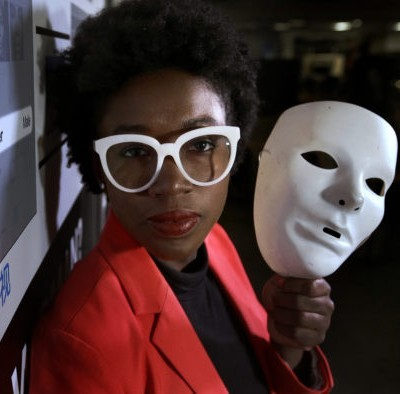
\includegraphics[width=1\textwidth]{./images/joy_buolamwini.jpg}
    \end{column}
    \begin{column}{0.7\textwidth}
        When Joy Buolamwini was a computer science undergrad at Georgia Tech in the early 2010s, she worked on an assignment to recognise emotions in faces. The problem was that the face recognition library she used would not detect her face, until she held up a white mask in front of her face.
        \\~\\
        At the time, many libraries were trained on the \emph{Labelled Faces in the Wild} database. It turned out that there are twice as many images of George W. Bush in the dataset as there are all of Black women combined.
    \end{column}
\end{columns}
\end{frame}

\begin{frame}
\frametitle{Face recognition and race 2}
\begin{columns}
    \begin{column}{0.4\textwidth}
        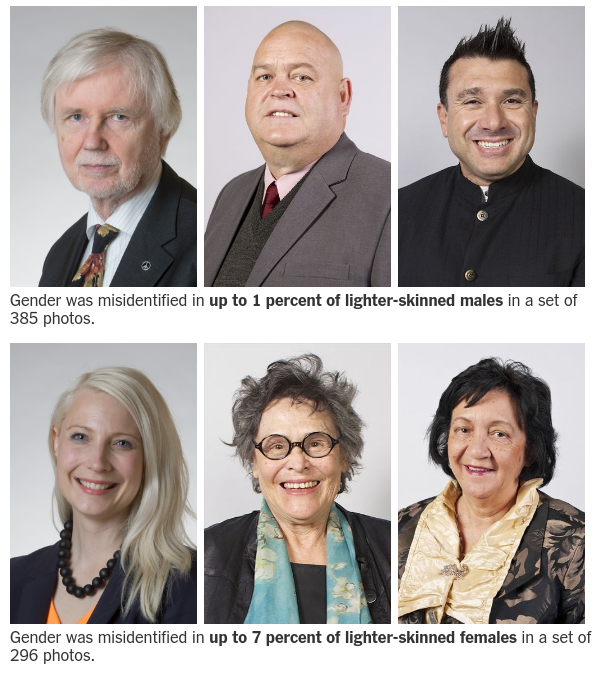
\includegraphics[width=1\textwidth]{./images/gender_race_1.png}
    \end{column}
    
    \begin{column}{0.4\textwidth}
        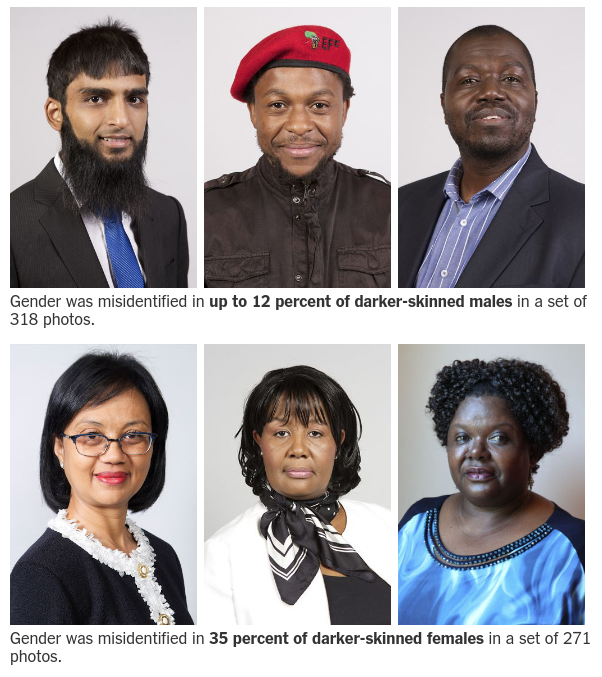
\includegraphics[width=1\textwidth]{./images/gender_race_2.png}
    \end{column}
\end{columns}
\small{Research by Joy Buolamwini and Timnit Gebru showed that the error rate of gender recognition was 100x higher for dark-skinned women than white men.}
\end{frame}

%% Word embeddings

\begin{frame}
\frametitle{The everyday sexism of word embeddings}


\begin{itemize}
    \item /emph{Word embeddings}, such as Word2Vec, encode words in space so that similar words are located together, and that relationships exist between words, such that:
    \begin{itemize}
        \item {Subtracting the word embedding vector for \textbf{male} from \textbf{king}, and adding the word vector for \textbf{female}, gives \textbf{queen}.}
    \end{itemize}
    \item{But these word embeddings learn relationships from human text.....}
        \begin{itemize}
        \item {Subtracting the word embedding vector for \textbf{male} from \textbf{doctor}, and adding the word vector for \textbf{female}, gives \textbf{nurse}.}
        \end{itemize}
    \item{Word embedding models are used in many text applications such as internet search, translation, and sentiment analysis.
    \item For discussion: What problems do you think could arise from biases in word embeddings?}
\end{itemize}

\end{frame}

%%%% Representation what can we learn

\begin{frame}
\frametitle{Representation - What can we learn?}
\begin{itemize}
\setlength{\itemsep}{5mm} % Increase spacing between bullets
    \item \textbf{Model performance is dependent on sufficient representation of examples in the dataset.}
    
    \item \textbf{Models should be tested for performance on subgroups}, especially when it is known there are sensitive groups (e.g. protected characteristics like gender and race) present.
    
    \item \textbf{The model builder is responsible for the data they use to build the model.} The buck stops with them. At a minimum they must identify and communicate key weaknesses in model performance (but better to try and fix them - by gathering more balanced data if possible, or reducing over-represented data).
\end{itemize}
\end{frame}




\end{document}